

% Gradient Info
  
\tikzset {_jtrrismjr/.code = {\pgfsetadditionalshadetransform{ \pgftransformshift{\pgfpoint{0 bp } { 0 bp }  }  \pgftransformscale{1 }  }}}
\pgfdeclareradialshading{_qh3cygrf7}{\pgfpoint{0bp}{0bp}}{rgb(0bp)=(1,0,0);
rgb(0bp)=(1,0,0);
rgb(11.607142857142858bp)=(1,1,1);
rgb(400bp)=(1,1,1)}

% Gradient Info
  
\tikzset {_a32pt6p6g/.code = {\pgfsetadditionalshadetransform{ \pgftransformshift{\pgfpoint{0 bp } { 0 bp }  }  \pgftransformscale{1 }  }}}
\pgfdeclareradialshading{_guvizw346}{\pgfpoint{0bp}{0bp}}{rgb(0bp)=(1,0,0);
rgb(0bp)=(1,0,0);
rgb(25bp)=(1,1,1);
rgb(400bp)=(1,1,1)}

% Gradient Info
  
\tikzset {_jarxx2wyd/.code = {\pgfsetadditionalshadetransform{ \pgftransformshift{\pgfpoint{0 bp } { 0 bp }  }  \pgftransformscale{1 }  }}}
\pgfdeclareradialshading{_yub9o70l6}{\pgfpoint{0bp}{0bp}}{rgb(0bp)=(1,0,0);
rgb(0bp)=(1,0,0);
rgb(25bp)=(1,1,1);
rgb(400bp)=(1,1,1)}

% Gradient Info
  
\tikzset {_a0dl0ojvx/.code = {\pgfsetadditionalshadetransform{ \pgftransformshift{\pgfpoint{0 bp } { 0 bp }  }  \pgftransformscale{1 }  }}}
\pgfdeclareradialshading{_okxfjrd6z}{\pgfpoint{0bp}{0bp}}{rgb(0bp)=(0,0,1);
rgb(0bp)=(0,0,1);
rgb(25bp)=(1,1,1);
rgb(400bp)=(1,1,1)}

% Gradient Info
  
\tikzset {_xpykvvipb/.code = {\pgfsetadditionalshadetransform{ \pgftransformshift{\pgfpoint{0 bp } { 0 bp }  }  \pgftransformscale{1 }  }}}
\pgfdeclareradialshading{_bmcdpxtb2}{\pgfpoint{0bp}{0bp}}{rgb(0bp)=(0,0,1);
rgb(0bp)=(0,0,1);
rgb(25bp)=(1,1,1);
rgb(400bp)=(1,1,1)}

% Gradient Info
  
\tikzset {_ws2f7c5v8/.code = {\pgfsetadditionalshadetransform{ \pgftransformshift{\pgfpoint{0 bp } { 0 bp }  }  \pgftransformscale{1 }  }}}
\pgfdeclareradialshading{_6mydlptux}{\pgfpoint{0bp}{0bp}}{rgb(0bp)=(1,0,0);
rgb(0bp)=(1,0,0);
rgb(25bp)=(1,1,1);
rgb(400bp)=(1,1,1)}

% Gradient Info
  
\tikzset {_e59aq2t28/.code = {\pgfsetadditionalshadetransform{ \pgftransformshift{\pgfpoint{0 bp } { 0 bp }  }  \pgftransformscale{1 }  }}}
\pgfdeclareradialshading{_qjz6rtgrj}{\pgfpoint{0bp}{0bp}}{rgb(0bp)=(1,0,0);
rgb(0bp)=(1,0,0);
rgb(25bp)=(1,1,1);
rgb(400bp)=(1,1,1)}
\tikzset{every picture/.style={line width=0.75pt}} %set default line width to 0.75pt        

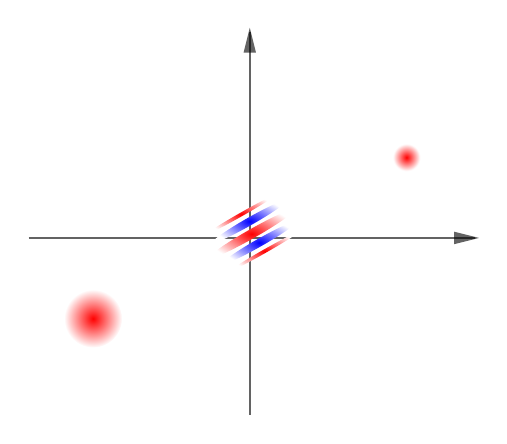
\begin{tikzpicture}[x=0.75pt,y=0.75pt,yscale=-1,xscale=1]
%uncomment if require: \path (0,300); %set diagram left start at 0, and has height of 300

%Straight Lines [id:da6137214521405325] 
\draw [color={rgb, 255:red, 0; green, 0; blue, 0 }  ,draw opacity=0.61 ]   (107.5,131.58) -- (322.5,131.58) ;
\draw [shift={(324.5,131.58)}, rotate = 180] [fill={rgb, 255:red, 0; green, 0; blue, 0 }  ,fill opacity=0.61 ][line width=0.08]  [draw opacity=0] (12,-3) -- (0,0) -- (12,3) -- cycle    ;
%Straight Lines [id:da585845343485853] 
\draw [color={rgb, 255:red, 0; green, 0; blue, 0 }  ,draw opacity=0.61 ]   (214,216.83) -- (214,32.33) ;
\draw [shift={(214,30.33)}, rotate = 450] [fill={rgb, 255:red, 0; green, 0; blue, 0 }  ,fill opacity=0.61 ][line width=0.08]  [draw opacity=0] (12,-3) -- (0,0) -- (12,3) -- cycle    ;
%Shape: Circle [id:dp9957208584958241] 
\draw  [draw opacity=0][shading=_qh3cygrf7,_jtrrismjr] (275.5,92.75) .. controls (275.5,85.02) and (281.77,78.75) .. (289.5,78.75) .. controls (297.23,78.75) and (303.5,85.02) .. (303.5,92.75) .. controls (303.5,100.48) and (297.23,106.75) .. (289.5,106.75) .. controls (281.77,106.75) and (275.5,100.48) .. (275.5,92.75) -- cycle ;
%Shape: Circle [id:dp2419944983168858] 
\draw  [draw opacity=0][shading=_guvizw346,_a32pt6p6g] (124.5,170.42) .. controls (124.5,162.68) and (130.77,156.42) .. (138.5,156.42) .. controls (146.23,156.42) and (152.5,162.68) .. (152.5,170.42) .. controls (152.5,178.15) and (146.23,184.42) .. (138.5,184.42) .. controls (130.77,184.42) and (124.5,178.15) .. (124.5,170.42) -- cycle ;
%Shape: Ellipse [id:dp5587895674427128] 
\draw  [draw opacity=0][shading=_yub9o70l6,_jarxx2wyd] (194.3,141.31) .. controls (193.68,140.22) and (202.4,134.11) .. (213.77,127.66) .. controls (225.14,121.2) and (234.86,116.85) .. (235.47,117.93) .. controls (236.09,119.02) and (227.37,125.13) .. (216,131.58) .. controls (204.63,138.04) and (194.91,142.39) .. (194.3,141.31) -- cycle ;
%Shape: Ellipse [id:dp13432105710862952] 
\draw  [draw opacity=0][shading=_okxfjrd6z,_a0dl0ojvx] (200.79,143.99) .. controls (200.27,143.08) and (207.86,137.8) .. (217.74,132.19) .. controls (227.62,126.58) and (236.05,122.77) .. (236.56,123.68) .. controls (237.08,124.59) and (229.49,129.88) .. (219.61,135.49) .. controls (209.73,141.1) and (201.3,144.9) .. (200.79,143.99) -- cycle ;
%Shape: Ellipse [id:dp12233431850576615] 
\draw  [draw opacity=0][shading=_bmcdpxtb2,_xpykvvipb] (196.11,133.74) .. controls (195.59,132.83) and (203.18,127.54) .. (213.06,121.93) .. controls (222.94,116.33) and (231.37,112.52) .. (231.89,113.43) .. controls (232.41,114.34) and (224.82,119.62) .. (214.94,125.23) .. controls (205.06,130.84) and (196.63,134.65) .. (196.11,133.74) -- cycle ;
%Shape: Ellipse [id:dp27990775863280604] 
\draw  [draw opacity=0][shading=_6mydlptux,_ws2f7c5v8] (193.38,129.63) .. controls (193.13,129.19) and (200.36,124.63) .. (209.52,119.43) .. controls (218.68,114.23) and (226.31,110.36) .. (226.55,110.8) .. controls (226.8,111.23) and (219.57,115.8) .. (210.41,121) .. controls (201.25,126.2) and (193.63,130.06) .. (193.38,129.63) -- cycle ;
%Shape: Ellipse [id:dp27120941544894017] 
\draw  [draw opacity=0][shading=_qjz6rtgrj,_e59aq2t28] (204.63,147.38) .. controls (204.38,146.94) and (211.61,142.38) .. (220.77,137.18) .. controls (229.93,131.98) and (237.56,128.11) .. (237.8,128.55) .. controls (238.05,128.98) and (230.82,133.55) .. (221.66,138.75) .. controls (212.5,143.95) and (204.88,147.81) .. (204.63,147.38) -- cycle ;




\end{tikzpicture}
